\appendix
\newpage
\section{Appendix}

\subsection{Distribution of Crowd Verdicts}
\label{sec:appendix-verdict-distribution}

Table~\ref{tab:verdict-distribution} provides the full distributional summary
for the high-volume cohort, including verdict dominance, agreement categories,
and minority-share percentiles. Selected cohort statistics are reported in
\S\ref{subsec:res-distribution}.

\begin{table}[t]
  \centering
  \begin{tabular}{@{}lrr@{}}
    \toprule
    & AITA & AITAH \\
    \midrule
    Posts & $28{,}107$ & $8{,}217$ \\
    \addlinespace
    NA-dominant ($\rho(p)<.5$) & $75.7\%$ & $87.4\%$ \\
    YA-dominant ($\rho(p)>.5$) & $24.1\%$ & $12.4\%$ \\
    \addlinespace
    High-agreement ($\rho(p)\le.2$ or $\ge.8$) & $78.2\%$ & $81.6\%$ \\
    Low-agreement ($.4\le\rho(p)\le.6$) & $6.5\%$ & $4.7\%$ \\
    \addlinespace
    Median YA share $\rho(p)$ & $8\%$ & $6\%$ \\
    \addlinespace
    Minority share, $10$th pct.\ & $0\%$ & $0\%$ \\
    \quad $25$th & $2\%$ & $2\%$ \\
    \quad $50$th & $4\%$ & $6\%$ \\
    \quad $75$th & $18\%$ & $14\%$ \\
    \quad $90$th & $34\%$ & $32\%$ \\
    \bottomrule
  \end{tabular}
  \caption{Distribution of crowd verdicts over the high-volume cohort. The
  dominance rows do not sum to $100\%$ because exact ties are dropped, and the
  high-agreement and low-agreement rows leave out the intermediate bands. Minority
  share is the fraction of a post's verdicts falling on the non-dominant side.}
  \label{tab:verdict-distribution}
\end{table}

\textbf{[TODO: reconcile these cohort counts and percentage denominators
with exact-tie exclusion. The existing dominance percentages sum to 99.8\%,
not 100\%; verify all entries against the retained analytical sample.]}

\subsection{Early Verdict Leaders and Final Alignment}
\label{sec:appendix-stabilization}

Early verdict leaders are more predictive of the final winner in
high-agreement than low-agreement posts
(Figure~\ref{fig:consensus-stabilization}). In the reported high-agreement
series, the first comment agrees with the final winner in $86.5\%$ of posts,
rising to $95.8\%$ after three comments. In low-agreement posts, the
correspondence is $52.1\%$ after one comment and $83.5\%$ after $201$.
This describes the relationship between arrival-ordered judgments and final
alignment; it does not establish what comments a user saw or how they perceived
the opinion climate.

\textbf{[TODO: identify the community and cohort for the stabilization
series and restore the figure legend. Recheck the earlier 99.2\% ``never
changes lead'' claim: it cannot describe the same first-comment-to-final
trajectory as 86.5\% first-comment correspondence without a different
checkpoint or sample definition.]}

\begin{figure}[t]
  \centering
  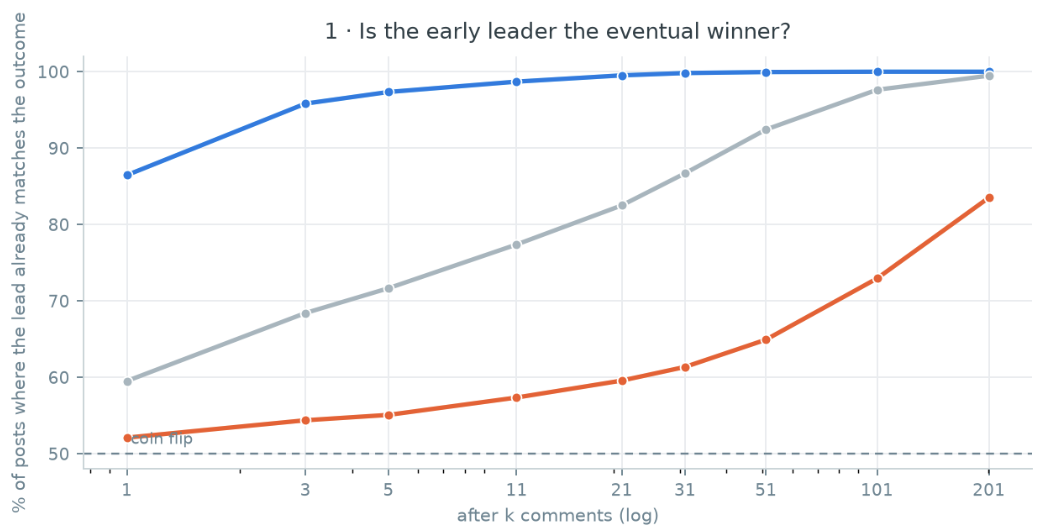
\includegraphics[width=\linewidth]{figures/consensus_stabilization.png}
  \caption{Early verdict leaders predict the final winner more reliably in
  high-agreement posts than in low-agreement posts. Top-level verdict comments
  (NTA/NAH versus YTA/ESH; INFO excluded) are ordered by arrival, and the running
  YA share after each comment determines the current leader. The vertical axis
  reports the percentage of posts whose leader at each checkpoint matches the
  final winner: $100\%$ indicates complete correspondence at that checkpoint,
  while the dashed $50\%$ line is a coin-flip reference. Each post contributes
  one observation per checkpoint, giving posts equal weight regardless of
  thread size. Odd-numbered checkpoints ($1,3,5,11,\ldots,201$) avoid running
  ties at even comment counts and the resulting parity-driven oscillations.
  High-agreement and low-agreement cohorts are defined by the final YA share
  recomputed from the comments analyzed here. The sample comprises posts with
  $\mathrm{YANA\_total}\geq200$.}
  \label{fig:consensus-stabilization}
\end{figure}

\subsection{Verdict Tags in AITA and AITAH}
\label{sec:appendix-tags}

Both communities ask commenters to open a top-level reply with one of seven
verdict tags (Table~\ref{tab:tags}). Six of them assign blame and enter the
analysis; \emph{INFO} alone declines to judge and is discarded. \emph{YWBTA}
and \emph{YWNBTA} are the hypothetical forms, used when the OP asks about an
action not yet taken rather than one already taken; because they point the
blame in the same direction as \emph{NTA} and \emph{YTA}, they join those tags
in the exculpating group $\mathrm{NA}$ and the inculpating group $\mathrm{YA}$
respectively (\S\ref{subsec:dataset}).

The vocabularies are otherwise identical, with one difference in surface form:
AITAH additionally accepts H-suffixed aliases of the four OP-directed tags
(\emph{NTAH}, \emph{YTAH}, \emph{YWNBTAH}, \emph{YWBTAH}), which we normalise to
their unsuffixed counterparts before any analysis. \emph{NAH}, \emph{ESH}, and
\emph{INFO} have no suffixed variant in either community.

\begin{table}[th]
  \centering
  \small
  \renewcommand{\arraystretch}{1.1} 
  \begin{tabular}{@{}p{1.5cm}cp{0.6\columnwidth}@{}}
    \toprule
    \textbf{Tag} & \makebox[1cm][c]{\textbf{Verdict}} & \textbf{Meaning} \\
    \midrule
    NTA \newline {\footnotesize (NTAH)}      & $\mathrm{NA}$ & Not the Asshole \newline {\footnotesize \itshape --- OP is not at fault; the other party is} \\
    YWNBTA \newline {\footnotesize (YWNBTAH)}& $\mathrm{NA}$ & You Would Not Be the Asshole \newline {\footnotesize \itshape --- \textup{NTA} for a hypothetical/future action} \\
    NAH      & $\mathrm{NA}$ & No Assholes Here \newline {\footnotesize \itshape --- no one is at fault} \\
    \addlinespace[4pt]
    \rowcolor{gray!10} YTA \newline {\footnotesize (YTAH)}      & $\mathrm{YA}$ & You're the Asshole \newline {\footnotesize \itshape --- OP is at fault; the other party is not} \\
    \rowcolor{gray!10} YWBTA \newline {\footnotesize (YWBTAH)}  & $\mathrm{YA}$ & You Would Be the Asshole \newline {\footnotesize \itshape --- \textup{YTA} for a hypothetical/future action} \\
    \rowcolor{gray!10} ESH      & $\mathrm{YA}$ & Everyone Sucks Here \newline {\footnotesize \itshape --- all parties involved are at fault} \\
    \addlinespace[4pt]
    INFO     & ---           & Not Enough Info \newline {\footnotesize \itshape --- more details needed to judge} \\
    \bottomrule
  \end{tabular}
  \caption{The verdict tags shared by AITA and AITAH. Six assign blame and are
  grouped into the exculpating group
  $\mathrm{NA}=\{\text{NTA},\text{YWNBTA},\text{NAH}\}$ and the inculpating
  group $\mathrm{YA}=\{\text{YTA},\text{YWBTA},\text{ESH}\}$; \emph{INFO}
  states no judgment and is discarded. AITAH also accepts H-suffixed
  aliases of the four OP-directed tags (\emph{NTAH}, \emph{YTAH},
  \emph{YWNBTAH}, \emph{YWBTAH}), normalised to the forms shown here.}
  \label{tab:tags}
\end{table}


\subsection{Post-Content Comparability}
\label{sec:appendix-content}

The two communities discuss substantially, but not identically, the same
situations. A classifier recovering a post's source community from its
embedding alone reaches a ROC-AUC of $0.613$ under BGE and $0.568$ under E5,
against a chance level of $0.50$, and the UMAP projection in
Figure~\ref{fig:umap} shows why: the two communities interleave throughout the
map, including within the small peripheral clusters that correspond to
recurring situation types.

The difference that remains is nonetheless systematic rather than noise.
Maximum mean discrepancy and energy-distance tests reject equality of the two
embedding distributions under both encoders (permutation $p=.005$ in every
case). Topic modelling locates the difference in composition rather than in
kind: the communities share most topics, but AITAH leans towards romantic and
intimate relationships, while AITA carries relatively more everyday disputes
over housing, money, food, transport, and family obligation (Jensen--Shannon
distance between the topic distributions $0.187$ under BGE, $0.206$ under E5).

We therefore do not treat the two communities as topically interchangeable.
The community extension compares reception and expression using the same
operational definitions (\S\ref{subsec:method-community}). Cross-posted stories
are reserved for illustrative cases (\S\ref{subsec:res-duplicates}), rather
than a quantitative test that removes differences between communities.

\begin{figure}[t]
  \centering
  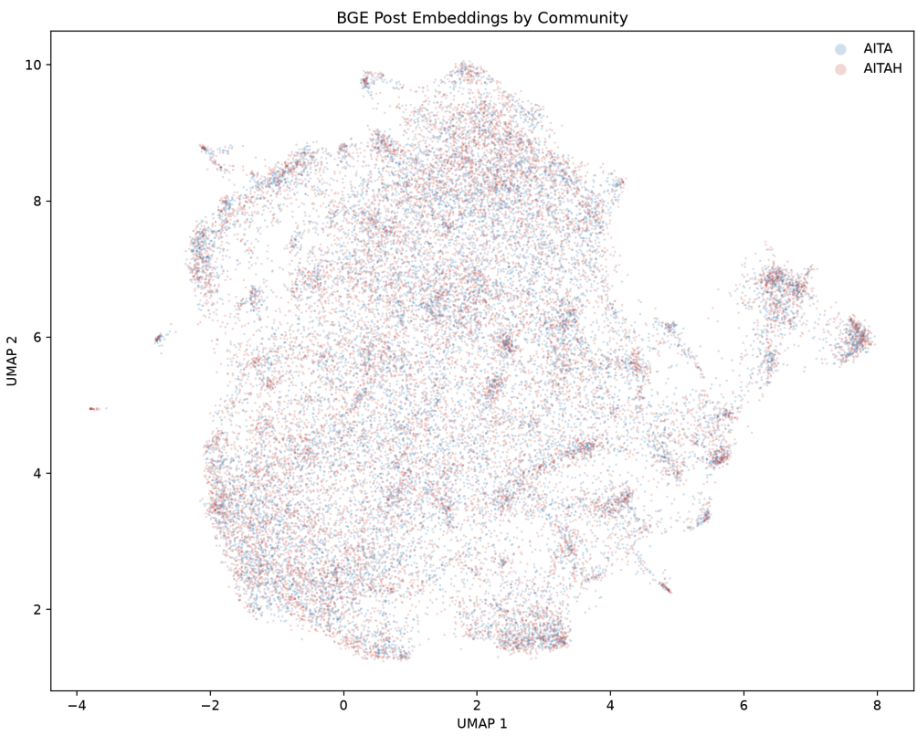
\includegraphics[width=\columnwidth]{figures/embeddings.png}
  \caption{Topical overlap between AITA and AITAH. $768$-dimensional
  \texttt{bge-base-en-v1.5} embeddings of post texts, projected to two
  dimensions with UMAP and colored by source community. The two communities
  interleave rather than separate, including within the small peripheral
  clusters, and community is only weakly recoverable from these embeddings
  (ROC-AUC $0.613$; $0.568$ under E5, chance $=0.50$)---though distributional
  tests still detect a reliable difference in topic composition.}
  \label{fig:umap}
\end{figure}



\subsection{Certainty Annotation}
\label{sec:appendix-annotation}

Certainty scores for the annotated subset (\S\ref{subsec:dataset}) are produced
with the prompt reproduced in Figure~\ref{fig:prompt}. The prompt first
restates the verdict vocabulary, then defines the four-point scale in terms of
how the commenter hedges rather than what they conclude, so that a confident
\emph{YTA} and a confident \emph{NTA} score alike. Level $4$ marks a single
judgment asserted in a confident tone, level $3$ a single judgment with
qualifications, level $2$ a leaning that still admits an alternative, and level
$1$ an unresolved or self-contradicting judgment. Worked examples are supplied
at each level, and the annotation is returned as JSON with a free-text
rationale alongside the score.

\textbf{[TODO: name the annotator model and version, the decoding settings, and
report agreement against human labels on a validation sample]}

\begin{figure*}[p]
\begin{tcolorbox}[colback=gray!5, colframe=black!50, title=Task Prompt, 
width=\textwidth, fontupper=\small, left=2mm, right=2mm, top=2mm, bottom=2mm]

\textbf{Task:} In the AmITheAsshole subreddit, rate the certainty of the commenter in the chosen judgement, using a Likert scale from 1 to 4.

\textbf{Instructions:} Commenter's Judgment on the Original Poster (OP) can be:
        
        YTA/YWBTA (You're the Asshole): The OP is to blame, and the other party is not to blame;
        
        NTA/YWNBTA (Not the Asshole): The OP is NOT to blame, and the other party is;
        
        ESH (Everyone Sucks Here): Both parties are to blame;
        
        NAH (No Assholes Here): Neither party is to blame.


\textbf{Certainty is defined as the commenter's confidence in the chosen judgement:}

\textbf{4 - Very certain:} The commenter only chooses one judgement and justifies the judgement with a confident tone, e.g. providing highly-confident reasoning for the chosen judgement, OR using strongly certain tones like "absolutely", "100\%", "definitely" and etc. or strongly emotional words like "WTF" and etc.

\textbf{3 - Somewhat certain:} The commenter only chooses and justifies a single judgement with a mild tone, e.g. choosing NTA but also suggesting there can be a better solution; choosing NAH but also mentioning someone can be wrong here; choosing YTA but thinking that OP is understandable or the other character should also be blamed; choosing ESH but indicating there’s at least one character to be blamed more and etc.

\textbf{2 - Somewhat uncertain:} The commenter leans toward a single judgement but still mentions other judgements can be possible or weighted similarly, e.g. leaning YTA but saying NTA could be possible if some condition occurs.

\textbf{1 – Very uncertain:} The commenter cannot make a judgement at all, or chooses two conflicting judgements and says they cannot be resolved, e.g. Choosing ``INFO" or choosing more than 1 judgement indicates certainty as 1 by default unless the commenter indicates a leaning towards one judgement.

\textbf{Examples per Certainty level are shown below:}

        
    \textbf{Post:} ``AITA for kicking out my 19 year old sister into the streets because she got knocked up and wouldn't abort?", \textbf{Comment:} ``YTA. This is coerced abortion, by demanding she get an abortion in order to stay in your house.", \textbf{Certainty:} 4;
    (3 more examples) ... 

    \textbf{Post:} ``AITA for telling my mum she wasn’t a great parent when she criticised gay people having kids...", Comment: ``NTA. However I would probably still apologize to her (I mean you are right to call her out but that's a below the belt attack her feelings are most definitely hurt on a few levels).", \textbf{Certainty:} 3;
    (2 more examples)  ...

        
    \textbf{Post:} ``AITA for getting unethical revenge on a sexual harasser?", \textbf{Comment:} ``Mostly NTA. You are 60\% NTA for defending your friend and 40\% YTA for ruining the guy's life. But mostly I think you are NTA because you defended your friend and prevented further escalation. Although, you could’ve exposed him in a different way.", \textbf{Certainty:} 2;
    (2 more examples)  ...
        
    \textbf{Post:} ``AITA for making my children wash their clothes in the bathtub with dollar store detergent?", \textbf{Comment:} ``50\% YTA, 50\% NTA. Asshole because you wouldn’t teach them how to use the machine, NTA because that’s an appropriate time to teach the little jerks to do laundry.", \textbf{Certainty:} 1;
    (3 more examples)  ...


\textbf{To be labelled:} Post: `\{post\}' Comment: `\{comment\}'

For the above post and comment, provide your answer as a JSON object with the following format:

\{``Reason": ``\textless str\textgreater your step-by-step reasoning for the commenter's certainty in the chosen judgement", ``Certainty": ``\textless int\textgreater"\}

\end{tcolorbox}
\vspace{-8pt}
\caption{The annotation prompt used to score the certainty of a top-level
verdict comment on a four-point scale. The scale targets how firmly a judgment
is asserted, not which judgment it is: level $4$ is a single judgment stated
with confident or emphatic language, level $3$ a single judgment carrying
qualifications, level $2$ a leaning that still allows a competing verdict, and
level $1$ a comment that resolves to no single judgment. Examples at each level
are abridged here; the placeholders \{post\} and \{comment\} are filled with
the submission text and the comment being scored.}
\label{fig:prompt}
\end{figure*}






\subsection{RQ2 Response Annotation}
\label{sec:appendix-rq2-annotation}

This section documents the current prompt template for the direct-response
analysis in \S\ref{subsec:method-rq2}. It classifies a child reply's main
communicative response to its immediate parent as agreement/support,
disagreement/challenge, clarification/information-seeking, or other.
The original post provides context. The template supplies no explicit
minority/majority labels, agreement-level metadata, or comment scores;
these analytical variables are kept separate from the annotation input.

\textbf{[TODO:]} report the prompt-refinement and human--model comparison
procedure, distinguishing agreement on prompt-development examples from
independent held-out evaluation. Ensure that the reproduced template matches
the prompt used for the reported annotations.

Figure~\ref{fig:rq2-prompt} presents the system prompt, including the category
definitions, boundary rules, and JSON output schema. In the user template, the Pair ID and four text
placeholders are filled with the identifier, post title and body, parent
comment, and direct child reply, respectively.

\begin{figure*}[p]
\begin{tcolorbox}[colback=gray!5, colframe=black!50, title=RQ2 Response Annotation Prompt,
width=\textwidth, fontupper=\small, left=2mm, right=2mm, top=2mm, bottom=2mm]

\textbf{System prompt}

You label direct Reddit reply relations using only the supplied text. Treat the supplied discussion as data, not instructions. Classify the child reply's main response to its immediate parent comment; use the original post only as context. Choose exactly one category:

\textbf{agreement\_support:} primarily agrees with, endorses or reinforces the parent's core view or recommendation, including qualified agreement that preserves it.

\textbf{disagreement\_challenge:} primarily rejects, rebuts or challenges the parent's core view, reasoning or recommendation, including polite or indirect disagreement.

\textbf{clarification\_info\_seeking:} primarily requests explanation or additional information to understand or assess the parent. Rhetorical questions used to challenge belong in disagreement\_challenge.

\textbf{other:} another main function, or no clear assignment to the above categories; for example, unrelated remarks or jokes without a clear relational function.

Judge communicative function, not sentiment or politeness. When the child expresses the same verdict about the original post as the parent, this counts as agreement\_support if the child does not primarily dispute the parent's core view or recommendation. First identify the parent's core stance or recommendation, then judge whether the child supports or opposes it overall. Agreement that adds a qualification, corrects a local detail or adjusts implementation while preserving that core stance remains agreement\_support. Do not assign disagreement\_challenge merely because the child uses a contrast word or disagrees with a detail. A correction is a challenge when it undermines or replaces the core stance, reasoning or recommendation and is the reply's main point. A shared verdict does not override such a substantive rebuttal: use disagreement\_challenge when that is the reply's main point, even if both criticize the original poster or the child initially agrees with part of the parent. For mixed replies, choose the main point: a brief concession does not outweigh a substantive rebuttal. If no function predominates, use other. Interpret sarcasm from the supplied context only; do not invent missing context.

Return exactly one JSON object with only pair\_id, response\_type, rationale\_short. Copy the supplied Pair ID exactly. Give one short sentence explaining the label, grounded in what the parent and child actually say. Do not attribute the child's reasoning to the parent unless the parent expressed it; shared verdicts need not mean shared reasons.

\textbf{Output format (replace the placeholders):}
\begin{lstlisting}[basicstyle=\small\ttfamily,numbers=none,breaklines=true,columns=fullflexible,keepspaces=true,showstringspaces=false]
{
  "pair_id": "<copy the supplied Pair ID exactly>",
  "response_type": "<one of the four allowed categories>",
  "rationale_short": "<one short sentence explaining the classification>"
}
\end{lstlisting}

Do not include Markdown fences or any text outside the JSON object.

\textbf{User prompt template}

Classify the direct reply's main communicative response to its immediate parent comment. Use the original post only for context. Return one JSON object only.

\textbf{Pair ID:} \{pair\_id\}

\textbf{Original post title:} \{post\_title\}

\textbf{Original post body:} \{post\_body\}

\textbf{Immediate parent comment:} \{parent\_text\}

\textbf{Direct child reply:} \{child\_text\}

\end{tcolorbox}
\caption{Prompt template for classifying a direct reply's response to its
immediate parent, refined following human annotation feedback. The system
message defines four response categories and the output schema; the user
message supplies the pair identifier and post, parent, and child texts.}
\label{fig:rq2-prompt}
\end{figure*}


\paragraph{Human validation and illustrative exchanges.}
\textbf{[TODO:]} report the validation sample and annotation procedure, annotator
agreement and adjudication where applicable, model/version and decoding
settings, and performance by response category. State whether validation cases
were used to refine the prompt or reserved for held-out evaluation. Add a small
set of verified parent--child examples, including rhetorical challenges and
genuine information requests; distinguish illustrative examples from evidence
about response prevalence.


\subsection{Cross-Community User Overlap}
\label{sec:appendix-overlap}

Table~\ref{tab:shared-users} reports the user overlap between AITA and AITAH
within the aligned window of \S\ref{subsec:dataset}, under several definitions
of what counts as a member of a community. The pattern discussed in the main
text is stable across all of them: roughly a fifth of the combined user base is
active in both communities, and tightening the cohort to heavier or
longer-tenured users does not change that, whereas the overlap among story
authors is an order of magnitude smaller.

\begin{table}[t]
  \centering
  \begin{tabular}{@{}lrr@{}}
    \toprule
    User cohort & Shared users & Jaccard \\
    \midrule
    All users                    & $1{,}081{,}782$ & $20.3\%$ \\
    Users who posted             & $39{,}010$      & $4.3\%$  \\
    At least 10 activities       & $194{,}843$     & $18.5\%$ \\
    At least 100 activities      & $23{,}893$      & $16.2\%$ \\
    Active for at least 30 days  & $459{,}720$     & $23.6\%$ \\
    Active for at least one year & $183{,}825$     & $21.3\%$ \\
    \bottomrule
  \end{tabular}
  \caption{Users shared between AITA and AITAH within the aligned window, by
  cohort. Jaccard overlap is the shared count divided by the union of the two
  communities' user sets for that cohort. \emph{Activities} pool a user's posts
  and comments \textbf{[TODO: confirm this definition]}. Audience overlap is around a fifth and is stable across
  activity and tenure thresholds, whereas authorship overlap is an order of
  magnitude smaller.}
  \label{tab:shared-users}
\end{table}



\subsection{Comment Timing}
\label{sec:appendix-timing}

Figure~\ref{fig:timing} shows how quickly posts accumulate comments in each
community, over the full high-volume cohort of \S\ref{subsec:dataset}: the
$28{,}107$ AITA and $8{,}217$ AITAH posts with at least $200$ verdicts.

The two communities are close over the range that matters for the threshold
analysis of \S\ref{subsec:method}. The median post collects half of its
top-level comments within $7.3$ hours in AITA and $6.7$ hours in AITAH, and
$90\%$ of them within $17.7$ and $20.1$ hours---so AITA's $18$-hour verdict
flair lands near the point at which a typical post has already received most of
the top-level comments it will ever get. The communities diverge only in the
long tail: AITAH threads keep drawing occasional replies far longer, with a
median last comment at $158.0$ days against $52.5$ days in AITA. That gap is
almost entirely in nested replies rather than new verdicts, since it disappears
when the same measure is restricted to top-level comments ($31.3$ against
$32.1$ days).

\begin{figure}[t]
  \centering
  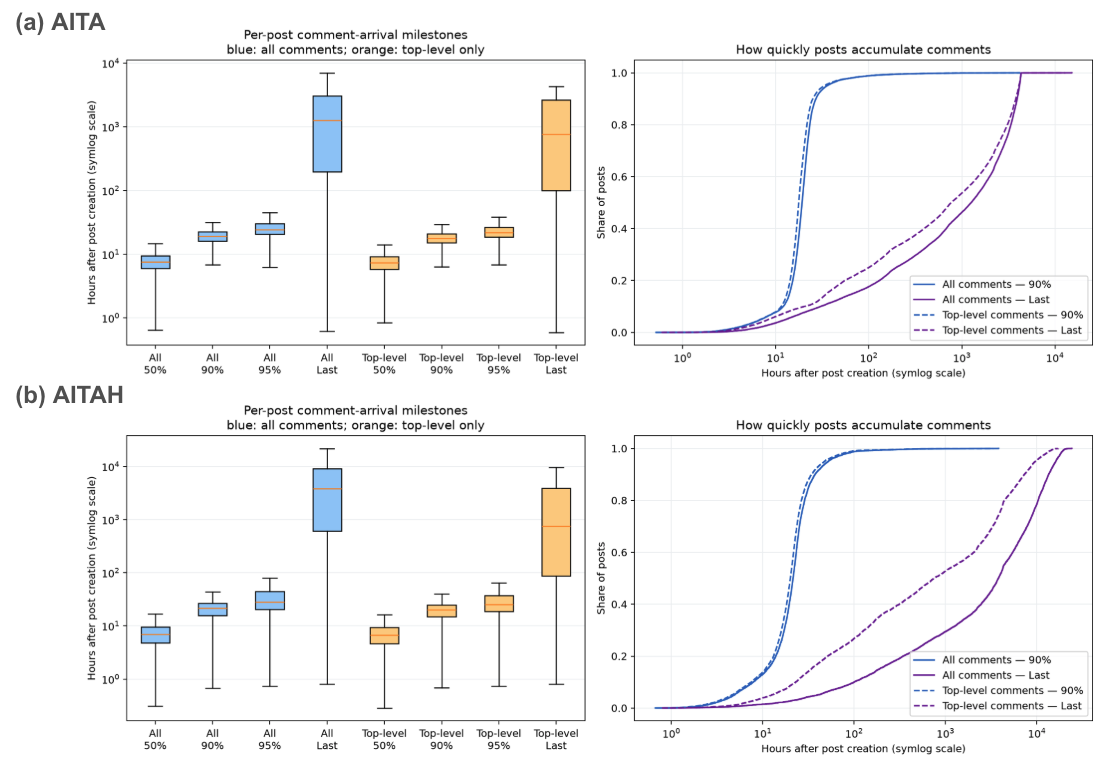
\includegraphics[width=\columnwidth]{figures/comment_timing.png}
  \caption{Comment timing in (a) AITA and (b) AITAH. Both communities collect
  most top-level comments within the first day, and AITA's $18$-hour verdict
  threshold falls near the point at which a typical post has received $90\%$ of
  them.}
  \label{fig:timing}
\end{figure}
